\documentclass[../manuscript.tex]{subfiles}
\section{Полученные результаты}
\begin{figure}[H]
\label{pic1.sec4}
    \centering
    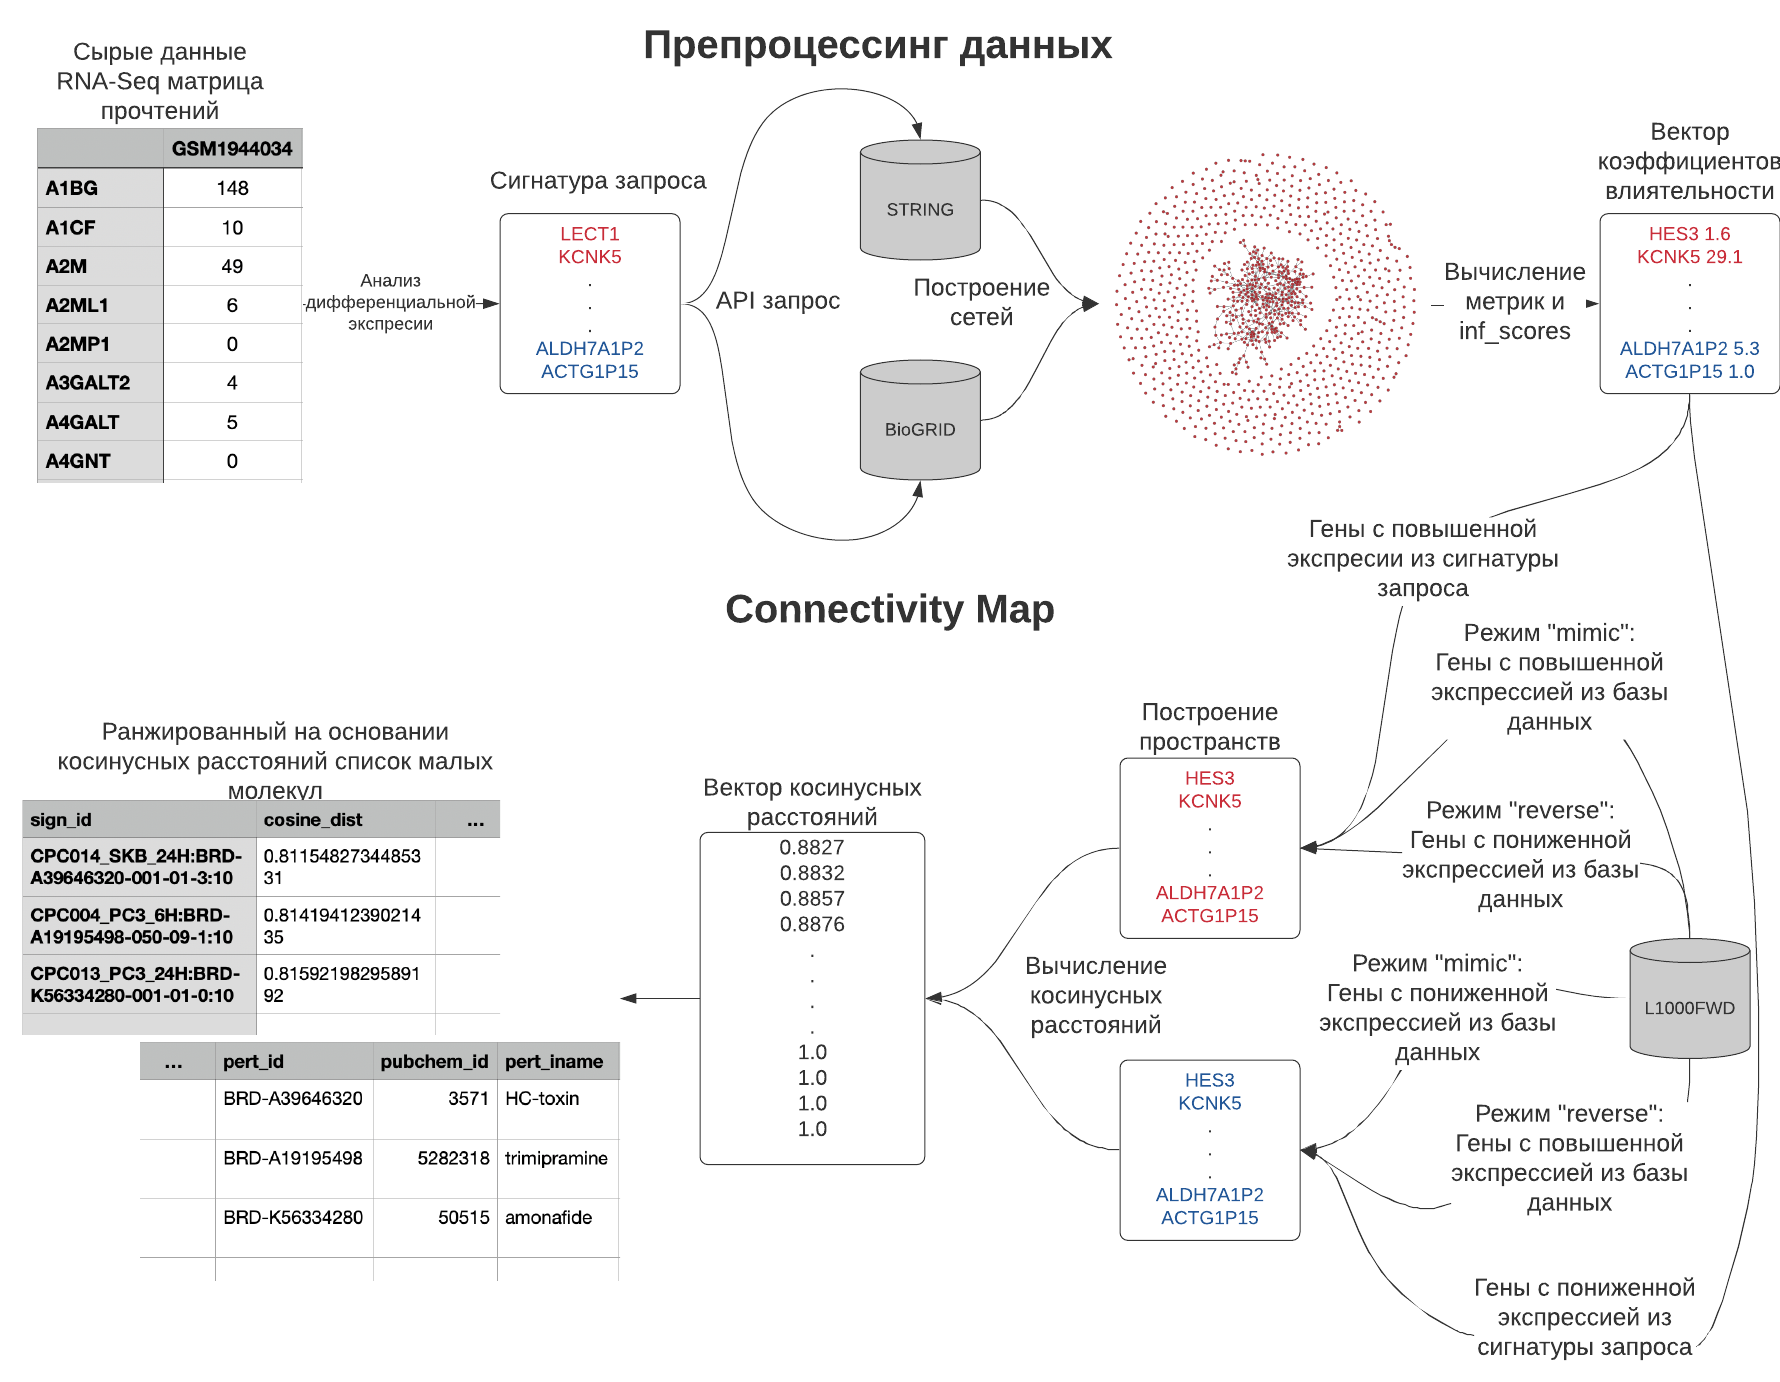
\includegraphics[scale=0.6]{pic_1_sec_4.png}
    \caption{Схема инструмента TopoCMap}
\end{figure}
\subsection{Структура подхода}
\par  TopoCMap - инструмент, разработанный, для проведения анализа Connectivity Map, который учитывает биологическую значимость генов в экспрессионной сигнатуре путем расчета так называемого коэффициента влиятельности для каждого дифференциально экспрессированного гена. В основе инструмента лежат различные этапы обработки данных, которые представлены на \hyperref[pic1.sec4]{рисунке выше}. Далее в этом разделе будет подробно описан каждый из них.
\subsubsection{Сырые данные и анализ дифференциальной экспрессии}
\par Используя фильтрацию генов по полученным в ходе анализа дифференциальной экспрессии  значениям $\log{FC}$ и $p\_value$, была получена экспрессионная сигнатура, состоящая из двух списков генов: генов с повышенной экспрессией (up) и генов с пониженной экспрессией (down). На этом этапе использовались следующие пороги по $\log{FC}$ и  $p\_value$: $|\log{FC}| \ge 1.5$ и $p\_value \le 10^{-3}$. Полученную сигнатуру будем в дальнейшем называть сигнатурой запроса. 
\subsubsection{Построение генных сетей и подсчет коэффициентов влиятельности}
\par Для оценки биологической значимости генов для определенного клеточного состояния, используется анализ сетей белок-белковых и ген-генных взаимодействий.

\subsubsection{Построение генных сетей}
\par На основании информации, полученной из STRING и BioGRID строятся генные сети. На основании построенных сетей рассчитываются топологические метрики центральности, такие как pagerank centrality (pr), betweenness centrality (bw), eigenvector centrality (ev), closeness centrality (cl), Katz centrality (kz), Hits centrality (hs), eigentrust (et). Метрики центральности позволяют определить так называемые белки-хабы, которые по сути являются наиболее связанными вершинами в сети белок-белковых взаимодействий. Эти метрики были выбраны на основе анализа ряда статей \cite{jeong2001, hahn2005, prvzulj2004, joy2005, park2009, wuchty2004, wunderlich2006}, в которых подробно описывается корреляция между этими метриками и важностью белков в сети белок-белковых взаимодействий. В перечисленных статьях также подробно описывалась летальность мутаций для клетки в одном из белков-хабов.
\subsubsection{Вычисление коэффициентов влиятельности}
\par Затем метрики центральности используются для расчета коэффициентов влиятельности для каждого гена в сигнатуре запроса. Также при вычислении коэффициентов влиятельности используется кратность изменения (FC), поскольку этот параметр количественно выражает степень изменения экспрессии гена. Предварительно FC были прологарифмированы, для уменьшения среднеквадратичного отклонения, а также нормализованы. Нормализация была проведена для унификации масштабов топологических метрик центральности, которые находятся в диапазоне от 0 до 1, и FC. Коэффициент влиятельности для гена i вычисляется как комбинация метрик:
$$
inf\_score_{i} = 
\begin{cases}
        (a_1 \cdot \log{FC} + b_1) \cdot (a_2 \cdot \textrm{pr} + b_2)\cdot(a_3 \cdot \textrm{bw} + b_3)\\ \cdot
        (a_4 \cdot \textrm{ev} + b_4) \cdot (a_5 \cdot \textrm{cl} + b_5) \cdot (a_6 \cdot \textrm{kz} + b_6) \\
        \cdot (a_7 \cdot \textrm{hs} +  b_7) \cdot (a_8 \cdot \textrm{et} + b_8) + a_9,\,\,\,\,\textrm{if gene in STRING}\\
    1, \,\,\,\, \text{otherwise}\\
\end{cases}
$$
где $a_1, a_2, b_1, b_2$ и тд. - числовые коэффициенты. Эти коэффициенты были подобраны на основании масштабной валидации на базе данных CFM \cite{cfm}, которая будет подробно описана ниже.

\subsubsection{Вычисление уровня сходства сигнатур}
\par В качестве сигнатур базы данных были взяты сигнатуры  LINCS, использовавшиеся в сходном инструменте L1000FWD \cite{l1000fwd}.
Оценка сходства сигнатуры запроса с сигнатурами базы данных рассчитывается как косинусное расстояние между генными векторами сигнатуры запроса и аналогичными векторами для сигнатуры из базы данных, усредненное для каждой пары. Генные вектора составляются следующим образом: генный вектор состоит из генов с повышенной (или пониженной) экспрессией, где на месте генов стоят коэффициенты влиятельности. Каждый генный вектор раскладывается по следующему пространству: гены из сигнатуры запроса + гены из сигнатуры базы данных. Таким образом, в позициях генного вектора могу стоять следующие величины:
\begin{itemize}
    \item $inf\_score_{i}$, если ген есть в раскладываемом списке и для него доступна информация о взаимодействиях в базах данных STRING или BioGRID
    \item 1, если ген есть в раскладываемом списке, но для него нет информации о взаимодействиях в базах данных STRING или BioGRID
    \item 0, во всех остальных случаях
\end{itemize}
\par На основании вычисленных косинусных расстояний ранжируются сигнатуры базы данных и, как следствие, малые молекулы, вызывающие такого рода изменения экспрессии. 
\subsubsection{Подбор коэффициентов для расчёта коэффициента влиятельности}

\par В этой главе будут подробно описаны все этапы валидации, приведенные на \hyperref[pic1.sec4.4]{рисунке ниже}. 
\begin{figure}[H]
\label{pic1.sec4.4}
    \centering
    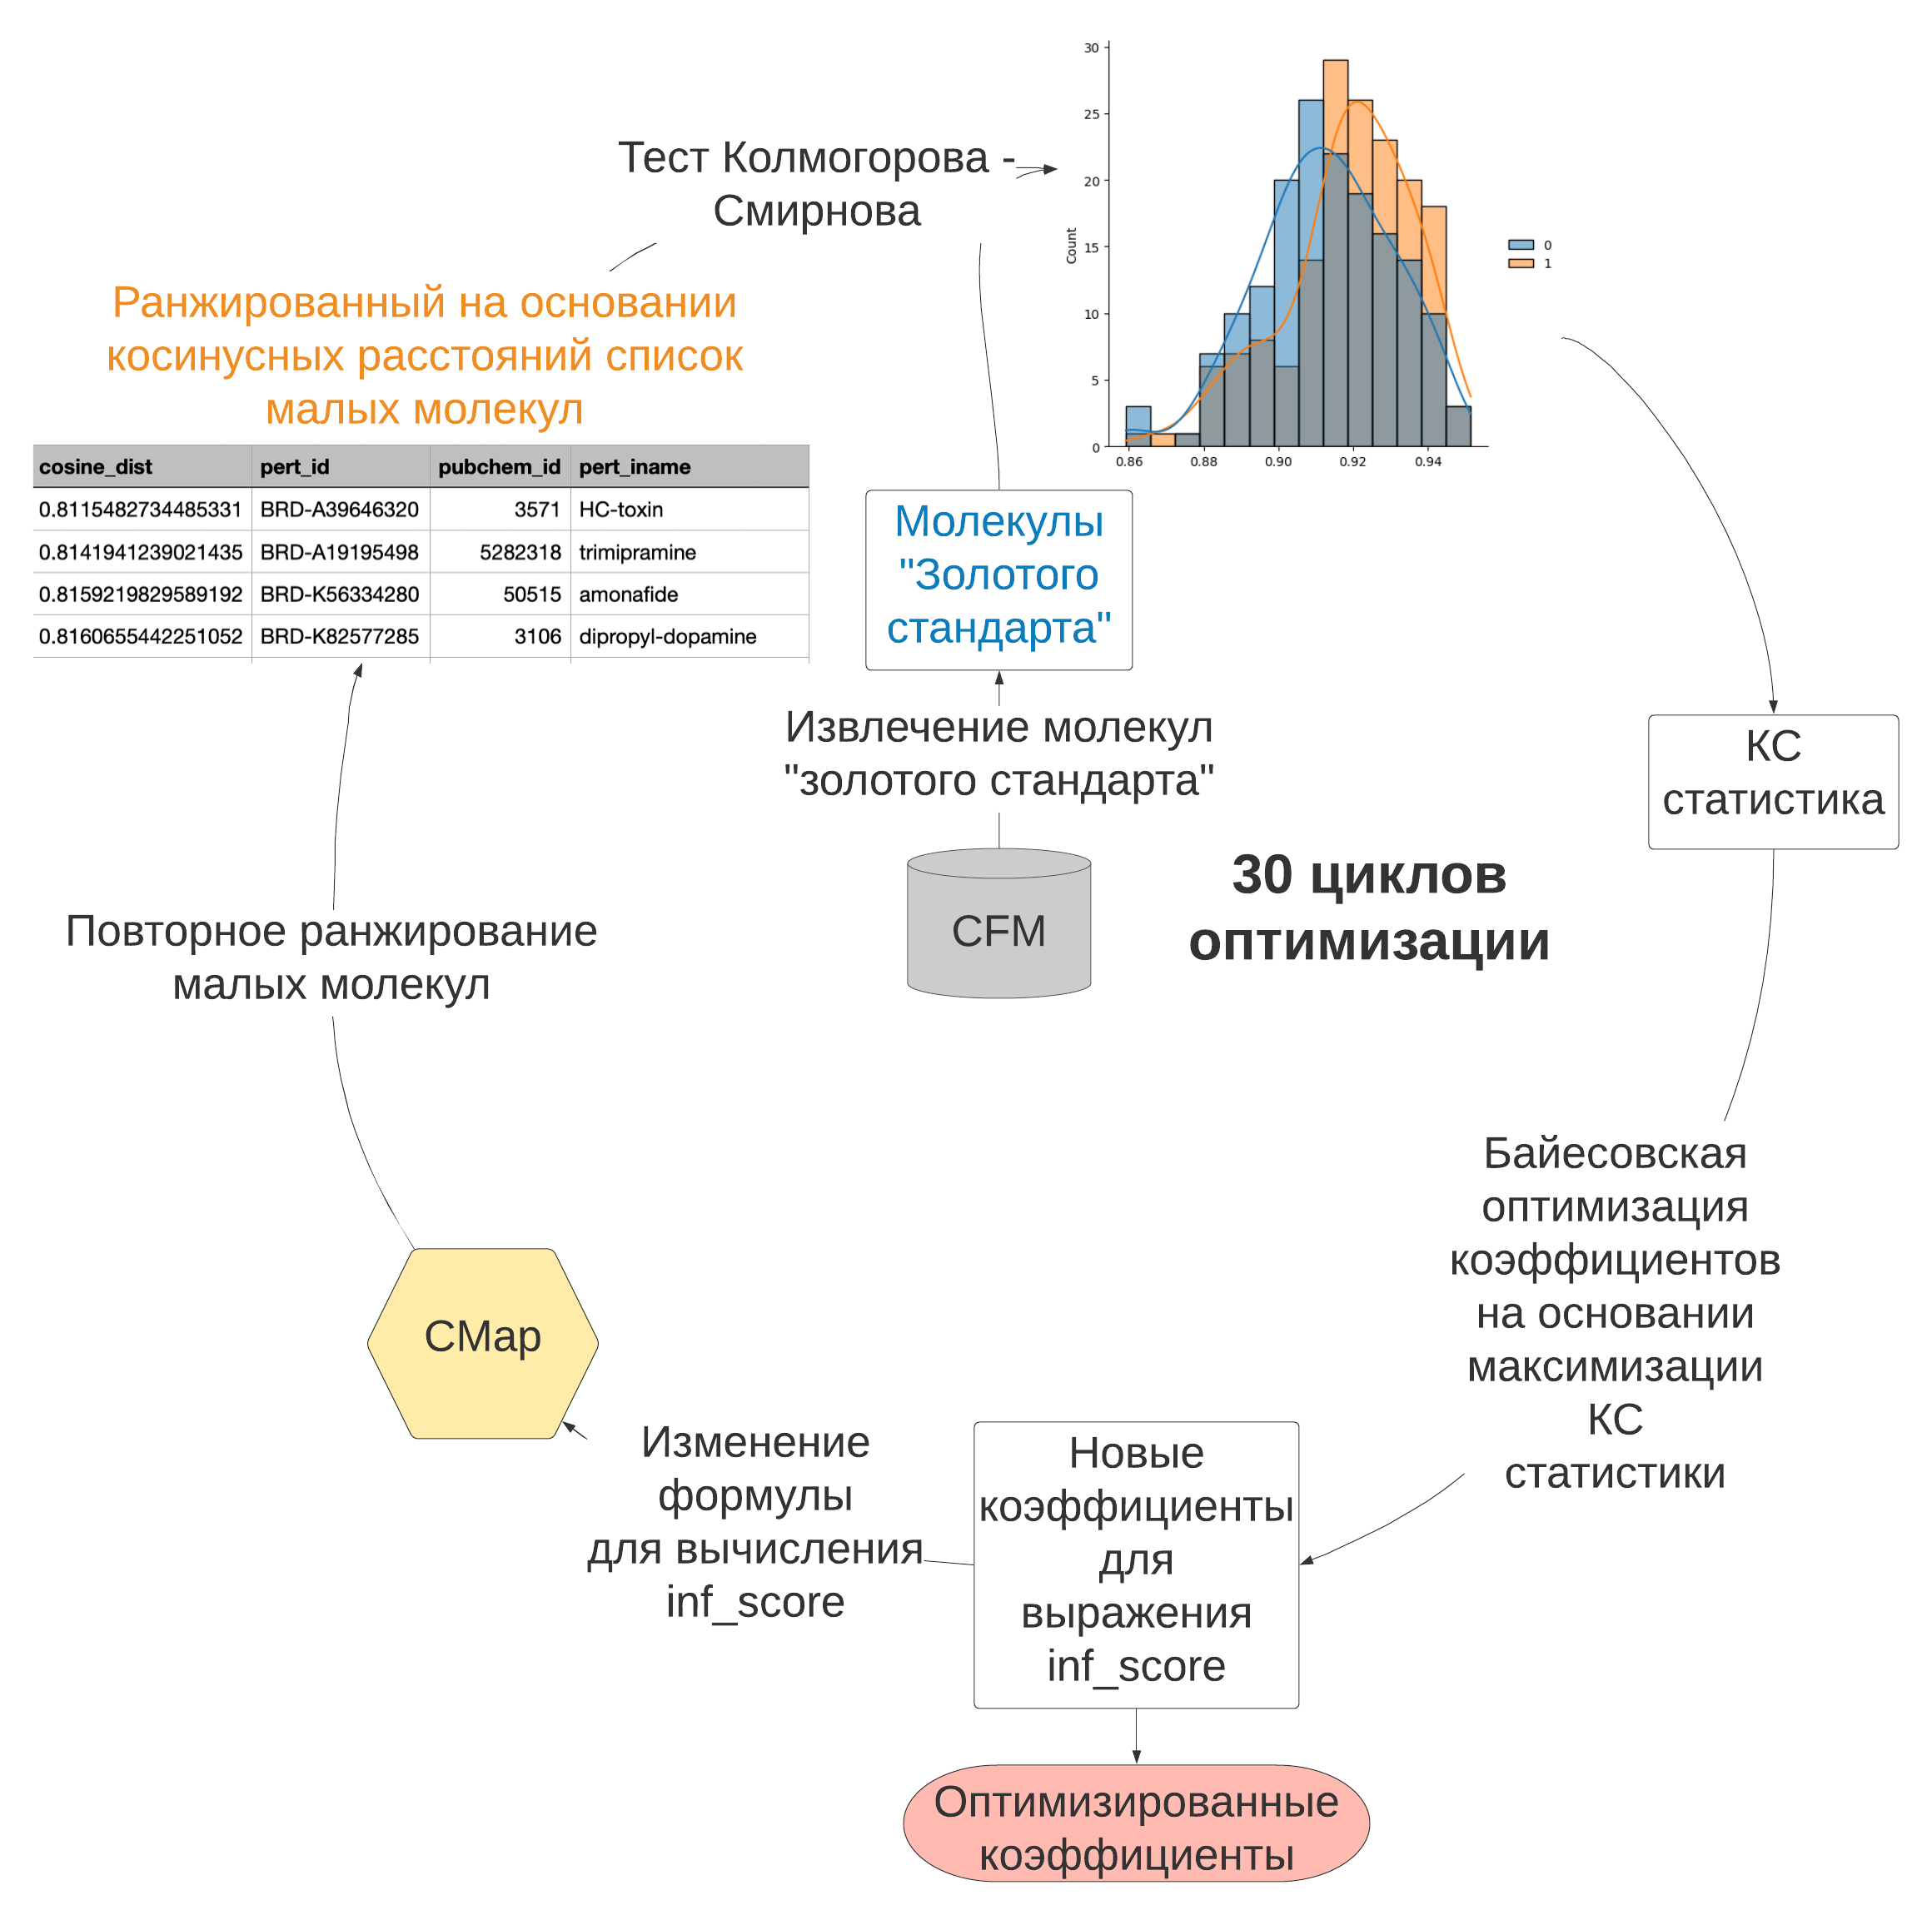
\includegraphics[scale=0.4]{pic_1_sec_4.4.png}
    \caption{Схема инструмента TopoCMap}
\end{figure}
\subsubsection{Извлечение молекул ''золотого стандарта''}

\par Для оптимизации необходимо сначала извлечь из доступных ресурсов некий ''золотой стандарт'', чтобы при последующей оптимизации была возможность оценивать точность модели. Для этих целей была использована база данных CFM \cite{cfm}, в которой содержится информация о малых молекулах, вызывающих трансдифференцировку между различными клеточными типами, например, фибробластами и кардиомиоцитами. В CFM содержится список экспериментальных протоколов из различных опубликованных исследований по химическому перепрограммированию клеток. Для каждого клеточного перехода был составлен список соединений ''золотого стандарта'', а также туда были добавлены молекулы похожие на соединения ''золотого стандарта''. Поиск таких соединений был осуществлен на основе данных, содержащихся в L1000FWD \cite{l1000fwd}. Сходство молекул вычислялось с помощью коэффициента Танимото, также известного как мера Жаккара.
\subsubsection{Оптимизация коэффициентов для расчета коэффициента влиятельности}
\par Для оптимизации коэффициентов в выражении для расчета коэффициента влиятельности была выбрана Байесовская оптимизация. Данный вид оптимизации был выбран, так как он наиболее хорошо подходит для поиска минимума аналитически неизвестной функции. В качестве функций минимизации была выбрана функция статистика Колмогорова-Смирнова, которая показывает расстояние между распределениями. В качестве анализируемых распределений рассматривались распределение косинусных расстояний случайного набора малых молекул, не являющихся ''золотым стандартом'', а также распределение косинусных расстояний для соединений из ''золотого стандарта'' для конкретного перехода. Метрика GSEA enrichment score \cite{gsea} использовалась для оценки качества ранжирования модели. В нашем случае мы использовали в качестве ранжированного списка - список всех малых молекул, ранжированный на основании косинусных расстояний, а в качестве выбранного - список молекул ''золотого стандарта'' для интересующего клеточного перехода. Байесовская оптимизация состояла из 30 итераций на 15 начальных точках. Результаты оптимизаций на различных клеточных переходах были усреднены и приняты за финальные коэффициенты влиятельности.


%%% Бывшие Результаты
\subsubsection{Результаты оптимизации}
Описанная в методах оптимизация производилась на шести трансдифференцировках, а именно:
\begin{itemize}
    \item Фибробласты (fb) $\rightarrow$ Индуцированные кардиомиоциты (heart)
    \item Фибробласты $\rightarrow$ Индуцированные нейроны (neuron)
    \item Фибробласты $\rightarrow$ Индуцированные нейральные стволовые клетки (neural)
    \item Фибробласты $\rightarrow$ Индуцированные панкреатические бета клетки (beta)
    \item Фибробласты $\rightarrow$ Индуцированные плюрипотентные стволовые клетки (ips)
    \item Мезенхимальные стволовые клетки (mes) $\rightarrow$ Индуцированные нейроны
\end{itemize}

\par В таблице \ref{num_of_protocoles_table} представлена статистика по каждому из переходов. Видно, что больше всего соединений и сигнатур было доступно для переходов из фибробластов в кардиомиоциты и нейроны.
Для каждого перехода, представленного в таблице \ref{num_of_protocoles_table}, в результате оптимизации был получен вектор оптимальных коэффициентов. В таблице \ref{coeffs_table} представлены оптимальные коэффициенты в зависимости от перехода.
\par После оптимизации для каждой клеточной конверсии был получен ранжированный список малых молекул, которые предположительно должны вызывать такой переход. Статистика по каждому переходу представлена в таблице \ref{val_stats_table}. Из этой таблице можно сделать вывод, что оптимизация оказалась наиболее удачной для перехода из фибробластов в индуцированные плюрипотентные стволовые клетки, так как большое количество соединений из ''золотого стандарта'' было приоритезировано методом, а также первое вхождение соединения ''золотого стандарта'' было на 20-ой позиции (tretinoin).

\begin{table}[H]
    \centering
    \caption{Статистика по трансдифференцировкам}
    \begin{tabular}{|c|c|c|c|}
    \hline
          Переход & \makecell{Протоколы} & \makecell{Количество\\ соединений из\\ ''золотого стандарта''} & \makecell{Количество сигнатур \\ для соединений  из\\ ''золотого стандарта''} & \hline
          
          \makecell{Фибробласты\\ $\downarrow$\\ Индуцированные\\ кардиомиоциты} & 19 & 42 & 3195& \hline
          
          \makecell{Фибробласты\\ $\downarrow$\\ Индуцированные\\ нейроны} & 8 & 27 & 1249& \hline
          
          \makecell{Фибробласты\\ $\downarrow$\\ Индуцированные\\ нейральные \\ стволовые клетки} & 6 & 17 & 1278& \hline
          
          \makecell{Фибробласты\\ $\downarrow$\\ Индуцированные\\ панкреатические \\ бета клетки} & 6 & 18 & 394& \hline
          
          \makecell{Фибробласты\\ $\downarrow$\\ Индуцированные\\ плюрипотентные \\ стволовые клетки} & 4 & 13 & 953& \hline
          
          \makecell{Мезенхимальные \\ стволовые клетки \\ $\downarrow$\\ Индуцированные \\ нейроны} & 5 & 14 & 548& \hline
    \end{tabular}
    \label{num_of_protocoles_table}
\end{table}

\begin{table}[H]
    \centering
    \caption{Оптимальные коэффициенты для каждого перехода}
    \begin{tabular}{|c|c|c|c|c|c|c|}
    \hline
          Метрика & \makecell{fb to \\heart} & \makecell{fb to \\neuron} & \makecell{fb to \\beta}&  \makecell{fb to \\ips}& \makecell{fb to \\neural}& \makecell{mes to \\neuron}&\hline
          
          logFC &  8,332&	9,981& 3,589&		1,725&	6,713&	1,0&\hline
          
          pagerank & 1,000&	4,821& 7,958&		4,682&	4,527&	7,125&\hline
          
          betweenness &	5,873&	8,342& 7,639&		7,977&	2,543&	9,464&\hline
          
          eigenvector&7,344&	10,0& 10,0&		3,511&	6,146&	4,890&\hline
          
          closeness	&
          1,0 &	10,0 &	10,0	&6,253&	1,625&	9,919&\hline
          
          katz &
          4,073&	1,102&	10,0	&2,196&	2,170&	6,324&\hline
          
          hits&
          1,060&	10,0 &	9,438	&1,178&	3,481&	9,475&\hline
          
          eigentrust &5,939&	8,487& 5,641&		9,412&	7,990&	3,988&\hline
          
          \makecell{Свободный \\член} &	1,0 &	0,544&	0,551	&0,722&	0,809&	0,665&\hline
    \end{tabular}
    \label{coeffs_table}
\end{table}
\begin{table}[H]
    \centering
    \caption{Результаты валидации для оптимальных коэффициентов для каждого перехода}
    \begin{tabular}{|c|c|c|c|c|c|c|}
    \hline
          \makecell{Метрика \\ качества} & \makecell{fb to \\heart} & \makecell{fb to \\neuron} & \makecell{fb to \\beta}&  \makecell{fb to \\ips}& \makecell{fb to \\neural}& \makecell{mes to \\neuron}&\hline
          
          \makecell{среднее значение\\ $p\_value$}&0,262&	0,531& 0,164 &		0,095&	0,370&	0,298	&\hline
          
          \makecell{$p\_value$  методом \\ GSEA} & 0,271&	0,0543& 	0,038	&0,061	&0,292	&0,096&\hline
          
          \makecell{Первое вхождение \\ соединения из \\ ''золотого стандарта''} &	207 &	587	& 121 &	20&	137&	526	&\hline
          
          \makecell{Количество соединений \\ ''золотого стандарта'' \\ в топ 5\% списка}&10&	10&  9&		15& 8 &	4&\hline
          
    \end{tabular}
    \label{val_stats_table}
\end{table}
\subsubsection{Результаты усреднения коэффициентов}
\par После проведенной оптимизации оптимальные для каждого перехода коэффициенты были усреденены. В результате получились следующие коэффициенты (таблица \ref{mean_coeffs_table}):
\begin{table}[H]
    \centering
    \caption{Усредненные оптимальные коэффициенты}
    \begin{tabular}{|c|c|c|c|c|c|c|c|c|}
    \hline
          logFC & pr &	bw & ev &		cl&	kz&	hs& et& \makecell{free\\coeff}&\hline
          5,233& 5,019& 6,973& 6,982& 6,466& 4,311& 5,772 & 6,909& 0,715&\hline
    \end{tabular}
    \label{mean_coeffs_table}
\end{table}
\par Исходя из полученных значений можно сделать следующие выводы: оптимальные коэффициенты, полученные для различных переходов слишком вариабельны - сложно сделать вывод, какая из метрик центральности вносит наибольший вклад; несмотря на большой разброс значений метрик, более приоритетными всё же являются метрики: eigenvector, betweenness, eigentrust, closeness.
\par Также была проведена валидация инструмента с усредненными коэффициентами для рассматриваемых переходов. Результаты валидации представлены в таблице \ref{val_mean_stats_table}.

\begin{table}[H]
    \centering
    \caption{Результаты валидации для усредненных коэффициентов для каждого перехода}
    \begin{tabular}{|c|c|c|c|c|c|c|}
    \hline
          \makecell{Метрика \\ качества} & \makecell{fb to \\heart} & \makecell{fb to \\neuron} & \makecell{fb to \\beta}&  \makecell{fb to \\ips}& \makecell{fb to \\neural}& \makecell{mes to \\neuron}&\hline
          
          \makecell{среднее значение\\ $p\_value$}&0,749&	0,552& 0,623 &		0,142&	0,484&	0,583	&\hline
          
          \makecell{$p\_value$  методом \\ GSEA} & 0,395&	0,153& 	0,116	&0,029	&0,182	&0,329&\hline
          
          \makecell{Первое вхождение \\ соединения из \\ ''золотого стандарта''} &	97 &	258	& 120 &	64&	84&	1029	&\hline
          
          \makecell{Количество соединений \\ ''золотого стандарта'' \\ в топ 5\% списка}&9&	6&  7&		11& 7 &	3&\hline
          
    \end{tabular}
    \label{val_mean_stats_table}
\end{table}
\par Видно, что после усреднения результаты немного ухудшились: возросло p\_value, уменьшилась статистическая значимость появления соединений ''золотого стандарта'' в топе ранжированного списка (p\_value, определенное методом GSEA уменьшилось), уменьшилось число соединений ''золотого стандарта'' в топ 5\%, однако примечательно, что ранг первого вхождения соединения из ''золотого стандарта'' возрос.
\par В целом, можно сделать вывод, что усреднение коэффициентов привело к ухудшению качества предсказаний модели, однако это не слишком искажает общую картину.

\subsection{Валидация инструмента}

\subsubsection{Анализ полученных списков для оптимальных коэффициентов}

\par Из-за того, что база данных CFM не на 100\% пересекается с базой сигнатур в ответ на малые молекулы L1000FWD, часть соединений ''золотого стандарта'' не могут быть отранжированы. Более того, каждое соединение встречается в списке более одного раза, так как в действительности инструмент ранжирует не вещества, а сигнатуры, вызванные этим веществом. Исходя из этого, полезно ввести метрику, такую как отношение количества соединений из пересечения CFM и L1000FWD в топ 5\% списка к общему числу молекул на пересечении CFM и L1000FWD для конкретного перехода. В таблице \ref{perc_in_gs_table} представлены результаты расчета данной метрики.
\begin{table}[h!]
    \centering
    \caption{Отношение числа соединений из ''золотого стандарта'' в топ 5\% к общему числу соединений из ''золотого стандарта''}
    \begin{tabular}{|c|c|c|c|c|c|}
    \hline
           \makecell{fb to \\heart} & \makecell{fb to \\neuron} & \makecell{fb to \\beta}&  \makecell{fb to \\ips}& \makecell{fb to \\neural}& \makecell{mes to \\neuron}&\hline
          
            \makecell{4 из 19 \\(21,1 \%)} & \makecell{5 из 10 \\(50\%)}&\makecell{5	из 11\\ (45,5\%)} & \makecell{4	из 8 \\(50\%)} & \makecell{2 из 5 \\(40\%)}&	\makecell{3 из 8 \\(37,5\%)}&\hline
          
    \end{tabular}
   \label{perc_in_gs_table}
\end{table}
\subsubsection{Поиск соединений по механизму действия}
\par Помимо этого, так как в качестве ''золотого стандарта'' используются соединения из протоколов статей по клеточным конверсия, то стоит предположить, что не все соединения с такого рода активностью вошли в наш ''золотой стандарт''. Для этого был проведен анализ механизмов действия для соединений ''золотого стандарта'' для каждого клеточного перехода. В таблицах \ref{moa_heart_gs_table} - \ref{moa_mes_neuron_gs_table} приведены механизмы действия соединений ''золотого стандарта''. Из этих таблиц можно сделать вывод, что наиболее распространенными механизмами действия для переходов являются:
\begin{itemize}
    \item Агонисты рецепторов ретиноевой кислоты и ингибиторы пути TGF-$\beta$ для перехода из фибробластов в кардиомиоциты
    \item Ингибиторы ДНК метилтрансфераз для перехода из фибробластов в панкреатические бета клетки
    \item Ингибиторы пути TGF-$\beta$ для перехода из фибробластов в нейроны
    \item Агонисты рецепторов ретиноевой кислоты для перехода из фибробластов в индуцированные плюрипотентные стволовые клетки
    \item Ингибиторы пути TGF-$\beta$ для перехода из фибробластов в нейральные стволовые клетки
    \item Ингибиторы пути TGF-$\beta$ для перехода из мезенхимальных стволовых клеток в нейроны
\end{itemize}
\par Также был проведен анализ механизмов действия соединений в топ 50 для каждого клеточного перехода. Таблицы анализа представлены в приложениях \ref{sup_tab_1} - \ref{sup_tab_6}.
Для большинства переходов, таких как: фибробласты - кардиомиоциты, фибробласты - панкреатические бета клетки, фибробласты - индуцированные плюрипотентные стволовые клетки, в топ 50 были найдены соединения с аналогичной активностью, что и активность некоторых соединений ''золотого стандарта''. Далее немного подробнее будут рассмотрены эти соединения.

\par Для перехода из фибробластов в бета клетки в топ 50 соединений были найдены вещества со следующими активностями: ингибиторы HDAC (HC-toxin, vorinostat, trichostatin-a). В топ 50 они встречаются 5 раз. Для этого перехода в ''золотом стандарте'' содержится ингибитор HDAC - romidepsin. Кроме того, в ''золотом стандарте'' есть ингибиторы GSK-3$\alpha/\beta$, ингибитор моноамин оксидазы, агонисты глюкокортикоидного рецептора и ингибиторы ДНК-метилтрансферазы. В топ 50 были найдены вещества с такой же активностью: TWS-119 (ингибитор GSK-3$\beta$), salsolinol (ингибитор моноамин оксидазы), beta\-methasone (агонист глюкокортикоидного рецептора), temozolomide(ингибиторы ДНК - метилтрансферазы).

\par Для перехода из фибробластов в кардиомиоциты в топ 50 соединений были найдены вещества со следующими активностями: ингибиторы GSK-3$\beta$ (NSC-693868, indirubin). Для этого перехода в ''золотом стандарте'' содержится ингибитор GSK-3$\beta$ - CHIR-99021. Кроме того, в ''золотом стандарте'' есть ингибиторы сигнального пути TGF-$\beta$. Хотя в топ 50 не нашлось ингибиторов TGF-$\beta$ и его рецепторов, в топ 50 нашлось большое количество ингибиторов белков-трансдукторов сигнала от TGF-$\beta$-рецептора. Например, TGF-$\beta$ запускает сигнальный путь NF$\kappa$B; в топ 50 был найден parthenolide, который является ингибитором сигнального пути NF$\kappa$B. Также TGF-$\beta$ запускает MAPK-киназный каскад посредством активации малой ГТФазы RAF, инструментом также были найдены 2 ингибитора RAF ГТФазы (SB-590885, GW-5074).


\begin{table}[H]
\caption{Механизм действия соединений ''золотого стандарта'' для перехода из фибробластов в кардиомиоциты}
\label{moa_heart_gs_table}
\begin{tabular}{|c|c|c|c|}
\hline
Ранг& CID & Название & \makecell{Механизм \\ действия}\\ \hline
93                             & 444795                   & Retinoic acid & \makecell{агонист рецептора ретиноевой кислоты}                                \\ \hline
587                            & 4521392                  & SB-431542     & \makecell{ингибитор пути\\ Activin/BMP/TGF-β}                          \\ \hline
951                            & 11238147                 & ICG-001       & ингибитор Wnt                                                    \\ \hline
987                            & 5289501                  & TTNPB         & \makecell{агонист рецептора ретиноевой кислоты}                                 \\ \hline
1316                           & 25150857                 & BIX-01294     & \makecell{ингибитор G9a \\гистон метилтрансферазы}                      \\ \hline
1498                           & 5092                     & rolipram      & \makecell{ингибитор\\ фофсодиестеразы типа 4 (PDE4)} \\ \hline
2810                           & 11524144                 & dorsomorphin  & \makecell{ингибитор ALK2, ALK6  и AMPK}                                   \\ \hline
3073                           & 448042                   & Y-27632       & \makecell{ингибитор ROCK1 и ROCK2}                                        \\ \hline
4460                           & 447966                   & LY-364947     & TGF-b сигнальный путь                                         \\ \hline
4718                           & 3121                     & valproic-acid & ингибитор гистон деацетилазы                                   \\ \hline
4951                           & 47936                    & forskolin     & CAMP агонист                                                       \\ \hline
7073                           & 9826528                  & PD-0325901    & ингибитор MEK/ERK сигнального пути                                       \\ \hline
9236                           & 9956119                  & CHIR-99021    & ингибитор GSK3β                                                  \\ \hline
\end{tabular}
\end{table}
\par Для перехода из фибробластов в индуцированные плюрипотентные стволовые клетки в топ 50 соединений были найдены вещества со следующими активностями: агонисты рецептора ретиноевой кислоты (fenretinide, isotretinoin, tretinoin). Для этого перехода в ''золотом стандарте'' содержатся агонисты рецептора ретиноевой кислоты - AM580, Retinoic acid. Кроме того, в ''золотом стандарте'' есть ингибиторы сигнального пути TGF-$\beta$. Хотя в топ 50 не нашлось ингибиторов TGF-$\beta$ и его рецепторов, в топ 50 нашлось большое количество ингибиторов белков-трансдукторов сигнала от TGF-$\beta$-рецептора. Например, TGF-$\beta$ запускает сигнальный путь NF$\kappa$B; в топ 50 был найден IKK-2-inhibitor-V, который является ингибитором сигнального пути NF$\kappa$B. Также TGF-$\beta$ запускает PI3K-Akt-киназный каскад посредством активации PI3K киназы, инструментом также были найдены 2 ингибитора PI3K киназы (wortmannin, AS-605240) и ингибитор Akt киназы (triciribine). В свою очередь Akt киназа активирует белковый комплекс mTORC, ингибитор которого также был найден инструментом (sirolimus). Аналогичные результаты были получены и для других трансдифференцировок.
\begin{longtable}[c]{|c|c|c|c|}
\caption{Механизм действия соединений ''золотого стандарта'' для \\перехода из фибробластов в бета клетки}
\label{moa_beta_cells_gs_table}
\hline
Ранг& CID & Название & \makecell{Механизм \\ действия}\\ \hline
13128  & 9444                              & Azacitidine & \makecell{ингибитор ДНК (цитозин-5)-\\метилтрансферазы 1}  \\ \hline                         & 5352062                           & Romidepsin                            & \makecell{селективный ингибитор \\гистон деацетилазы}                     \\ \hline
& 5222465                           & Sodium butyrate                        & холинэстераза                      \\ \hline
& 19493                             & Parnate                              & \makecell{ингибитор моноамин оксидазы}                               \\ \hline
601                                             & 702558                            & RG-108                                                                           & \makecell{RG108 ингибитор\\ ДНК метилтрансферазы}                   \\ \hline
2150                                            & 9956119                           & CHIR-99021                                                                       & \makecell{ингибитор GSK-3α и GSK-3β;\\ ингибитор киназы\\ гликоген синтазы}                               \\ \hline
5091                                            & 222786                            & Cortisone                                                                        & \makecell{агонист глюкокортикоидного\\ рецептора;\\индуктор аннексина 1}              \\ \hline
\multicolumn{1}{|l|}{}                          & 24776445                          & Vismodegib                                                                       & \makecell{ингибитор трансмембранного \\белка-гомолога Smoothened\\(SMO) в сигнальном\\ пути Hedgehog}       \\ \hline
1448                                            & 25195294                          & LDN-193189                                                                       & \makecell{селективный\\ ингибитор ALK2 и ALK3}              \\ \hline
15909                                           & 936                               & Nicotinamide                                                                     &\makecell{ продукт АДФ-рибозил \\циклазы 2} \\ \hline
2652                                            & 25150857                          & BIX-01294                                                                        & \makecell{ингибитор гистон\\ метилтрансферазы}                       \\ \hline
889                                             & 444795                            & Tretinoin                                                                        & \makecell{природная\\ производная витамина A}                  \\ \hline
86                                              & 24775005                          & Erismodegib                                                                      & \makecell{ингибитор сигнального \\ пути Hedgehog}                     \\ \hline
\multicolumn{1}{|l|}{}                          & 10990876                          & \makecell{Sodium ascorbyl\\ phosphate}                                                        & синтетическая форма витамина C                              \\ \hline
1892                                            & 5743                              & Dexamethasone                                                                    & \makecell{агонист глюкокортикоидного\\ рецептора; стимулятор ядерного \\рецептора; агонист аннексина A1;\\  индуцибельный отрицательный \\модулятор синтазы оксида азота} \\ \hline
\end{longtable}
\begin{table}[h]
\caption{Механизм действия соединений ''золотого стандарта'' для перехода из фибробластов в нейроны}
\label{moa_neuron_gs_table}
\begin{tabular}{|c|c|c|c|}
\hline
Ранг& CID & Название & \makecell{Механизм \\ действия}                                                                             \\ \hline
\multicolumn{1}{|l|}{}         & 52912189                                              & I-BET151     & Inhibitor of the BET family                                                      \\ \hline
1366                           & \multicolumn{1}{l|}{448042}   & Y-27632      & Inhibitor of ROCK1 and ROCK2  \\ \hline
\multicolumn{1}{|l|}{}         & 16047442                                              & KC7f2        & Inhibitor of HIF 1-alpha                                                         \\ \hline
5935                           & 4521392                                               & SB431542     & Sonic hedgehog                                                                   \\ \hline
742                            & \multicolumn{1}{l|}{25195294} & LDN193189    & Inhibitor of TGF-beta/Smad signaling                                             \\ \hline
1533                           & 4878                                                  & PP2          & \makecell{активатор SIRT1 и \\ингибитор  аминоресвератолсульфата\\ и Src киназы} \\ \hline
\multicolumn{1}{|l|}{}         & 449054                                                & RepSox       & \makecell{ингибитор ALK5 \\(рецептор TGF-β типа 1) }                                   \\ \hline
556                            & 11524144                                              & Dorsomorphin & ингибитор ALK2, ALK6  и AMPK                                                \\ \hline
1547                           & 19582717                                              & ISX9         & 
Нейрогенный модулятор                                                             \\ \hline
9517                           & 47936                                                 & Forskolin    & CAMP агонист                                                                    \\ \hline
\end{tabular}
\end{table}

\begin{table}[H]
\caption{Механизм действия соединений ''золотого стандарта'' для перехода из фибробластов в индуцированные плюрипотентные стволовые клетки}
\label{moa_ips_gs_table}
\begin{tabular}{|c|c|c|c|}
\hline
Ранг& CID & Название & \makecell{Механизм \\ действия}\\ \hline
9839                           & 5743                     & Dexamethasone          & \makecell{активатор глюкокортикоидного\\ пути}               \\ \hline
\multicolumn{1}{|l|}{}         & 56962337                 & SGC0946                & \makecell{ингибитор DOT1L\\ метилтрансферазы }         \\ \hline
\multicolumn{1}{|l|}{}         & 19493                    & Parnate                & \makecell{ингибитор лизин-специфической\\ 
деметилазы 1 (LSD1)} \\ \hline
\multicolumn{1}{|l|}{}         & 449054                   & RepSox                 & \makecell{ингибитор ALK5 \\(рецептор TGF-β типа 1)  }   \\ \hline
1150                           & 47936                    & Forskolin              & агонист CAMP                                     \\ \hline
334                            & 2126                     & AM580                  & \makecell{агонист рецептора\\ ретиноевой кислоты}             \\ \hline
1092                           & 451668                   & 5-Aza-2'-deoxycytidine & ингибитор метилирования ДНК                    \\ \hline
20                             & 444795                   & Retinoic acid          & \makecell{агонист рецептора\\ ретиноевой кислоты}               \\ \hline
\end{tabular}
\end{table}
\begin{table}[h]
\caption{Механизм действия соединений ''золотого стандарта'' для перехода из фибробластов в индуцированные нейральные стволовые клетки}
\label{moa_neural_gs_table}
\begin{tabular}{|c|c|c|c|}
\hline
Ранг& CID & Название & \makecell{Механизм \\ действия}\\ \hline
1190 & 25150857                 & BIX01294    & \makecell{ингибитор G9a гистон\\ метилтрансферазы} \\ \hline
3070 & 702558                   & RG108       & \makecell{ингибитор ДНК\\ метилтрансферазы}         \\ \hline
                           & 46209426                 & Thiazovivin & \makecell{ингибитор RHO/ROCK\\ сигнального пути}              \\ \hline
137  & 25195294                 & LDN193189   & \makecell{Ингибитор TGF-beta/Smad\\ сигналинга}           \\ \hline
                           & 449054                   & RepSox      & \makecell{Ингибитор ALK5 \\(рецептор TGF-β типа 1)}  \\ \hline
\end{tabular}
\end{table}
\newpage
\begin{table}[h]
\caption{Механизм действия соединений ''золотого стандарта'' для перехода из мезенхимальных стволовых клеток в индуцированные нейроны}
\label{moa_mes_neuron_gs_table}
\begin{tabular}{|c|c|c|c|}
\hline
Ранг& CID & Название & \makecell{Механизм \\ действия}\\ \hline             
                           & 52912189                 & I-BET151     & ингибитор семейства BET                   \\ \hline
1124 & 47936                    & Forskolin    & агонист CAMP                                  \\ \hline
4230 & 4521392                  & SB431542     & ингибитор Activin/BMP/TGF-β пути    \\ \hline
526  & 448042                   & Y-27632      & ингибитор ROCK1 и ROCK2                  \\ \hline
                           & 5288382                  & Geldanamycin & ингибитор белка теплового шока 90        \\ \hline
                           & 9687                     & Bucladesine  & активатор пути CAMP                        \\ \hline
4437 & 11524144                 & Dorsomorphin & ингибитор ALK2, ALK3, ALK6 и AMPK        \\ \hline
                           & 449054                   & RepSox       & ингибитор ALK5 (рецептор TGF-β типа 1) \\ \hline
\end{tabular}
\end{table}
\newline
\subsubsection{Сравнение инструмента с инструментом Connectivity Map}
\par В ходе проделанной работы были проведены тесты инструмента на сигнатурах из статьи Lamb et al.\cite{lamb2006}.
Инструмент был опробован на 11 следующих сигнатурах:
\begin{itemize}
    \item Сигнатура S1 - клетки T24 (мочевой пузырь), MDA 435 (карцинома груди) и MDA 468 (карцинома груди), обработанные тремя ингибиторами гистондеацетилазы (HDAC): вориностатом (также известным как субероиланилидгидроксамовая кислота или SAHA), MS -27-275 и трихостатином А
    \item Сигнатура S2 - клетки MCF7 обрабатывали лигандом природного рецептора эстрогена (ER), 17$\beta$-эстрадиолом (E2)
    \item Сигнатура S3 - из пяти сигнатур в ответ на 5 различных фенотиазинов была создана одна сигнатура из генов, регулируемых всеми пятью соединениями (thioridazine, chlorpromazine, fluphenazine, trifluoperazine и prochlorperazine)
    \item  Сигнатура S4 - сигнатура S6 - альтернативные внутренние фенотиазиновые сигнатуры
    \item  Сигнатура S7 - сигнатура гедонина при лечении этим соединением клеток рака простаты LNCaP в течение 6 часов
    \item  Сигнатура S8 - агонисты PPARγ, связанные с ожирением, вызванным специфическим питанием у крыс
    \item Сигнатура S9 - Сигнатура S10 - DAPH как потенциальное терапевтическое средство против AD
    \item Сигнатура S11 - чувствительности к дексаметазону, полученная путем сравнения лейкозных клеток костного мозга пациентов, проявляющих либо чувствительность к дексаметазону, либо резистентность к нему in vitro
\end{itemize}
\par Инструмент TopoCMap показал высокое качество предсказаний на данных сигнатурах. 
Так для сигнатуры S1 топ 100 молекул полученного списка имели активность ингибиторов HDAC, для сигнатуры S7 gendanamycin, который обладает аналогичной активностью, что и gedunin, встречается в топ 100 списка 8 раз. Аналогичные результаты были получены и для остальных сигнатур.
\par На рисунке \ref{pic1.sec5.4} схематически представлены 2 ранжированных списка малых молекул, полученных для сигнатур S1 (слева) и S7 (справа), описанные выше.
\begin{figure}[H]
    \centering
    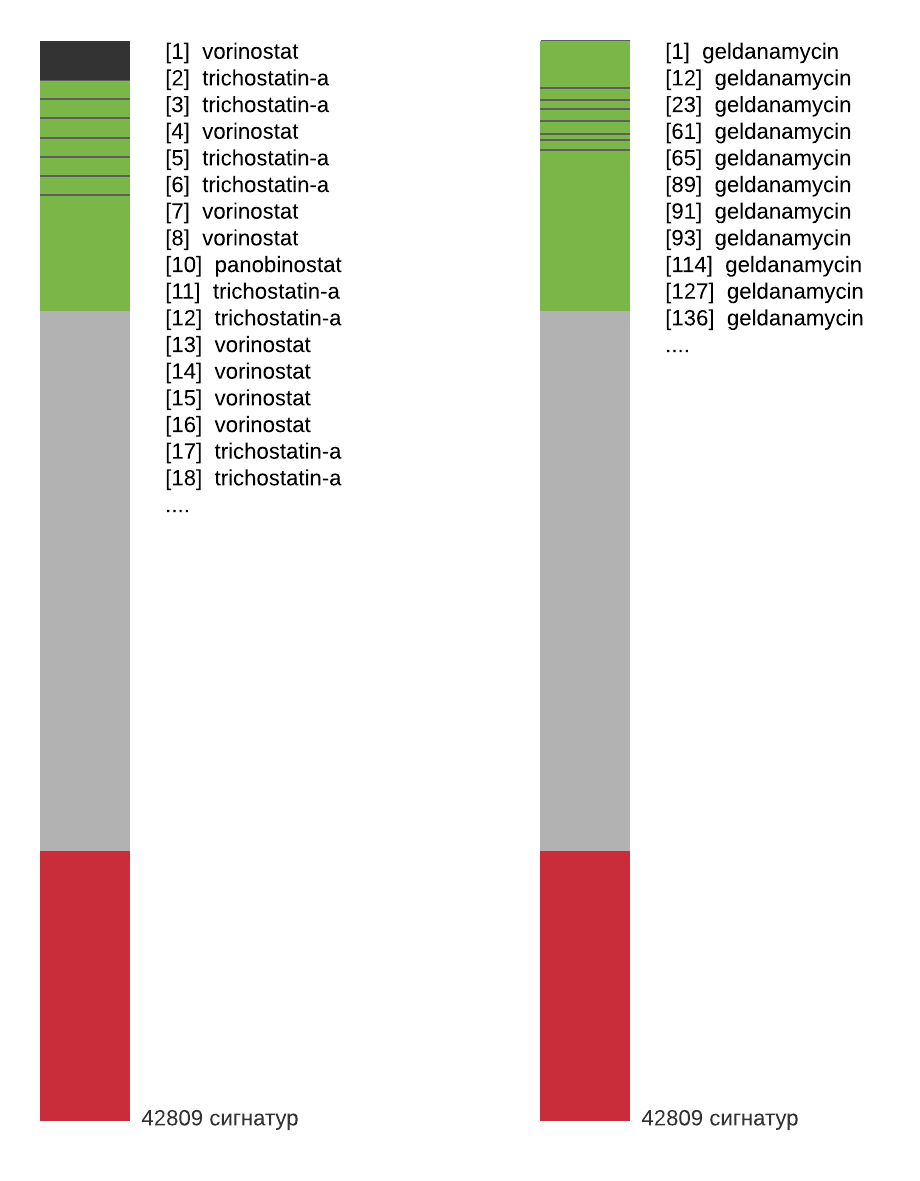
\includegraphics[scale=0.7]{pic_1_sec_5.4.png}
    \caption{Схематичное представление ранжированных списков малых молекул для сигнатур S1 (слева) и S7 (справа)}
    \label{pic1.sec5.4}
\end{figure}
\par В базе сигнатур, применяющейся Lamb et al., было 453 сигнатур, большинство из которых были сигнатурами в ответ на соединения интереса из статьи. Также в этой базе сигнатур содержалось всего 3 клеточные линии, которые были весьма схожи по своей биологии, и одно время обработки.  
\par  В базе сигнатур TopoCMap содержится 42809 сигнатур в ответ на более чем 4000 соединений. Также в этой базе анализируется большое количество клеточных линий, различное время обработки химическими агентами, а также большое количество биологических копий экспериментов.
\par Из-за столь существенных различий между базами сигнатур инструмента TopoCMap и инструмента, описанного в статье Lamb et al., количественное сравнение подходов затруднено. 